\clearpage
\subsection{Motor}
\label{subsec:Motor}

Um ein Glas während der Zubereitung hin- und her zu bewegen, wird eine Antriebsgruppe benötigt. Die Auswahl der Motorengruppe wurde mehr oder weniger vom Dozenten vorgegeben. Der Entscheid fiel dabei auf den Brushless DC-Motor AKM22h von Sigmatec. Auch dessen Ansteuerung ergab sich durch die schon vorhandenen EVAL-Boards mit TMC4671 und UPS 10A70V. Das benötigte Feedback wird vom ABN-Encoder AMT33 von CUI devices verwendet. Auf die erwähnten Komponenten wird im Folgenden eingegangen. Äbbildung \ref{fig:Blockdiagramm_TMC4671_und_TMC6200} zeigt, wie die ICs zusammenhängen. 

\begin{figure}[h!]
	\centering
	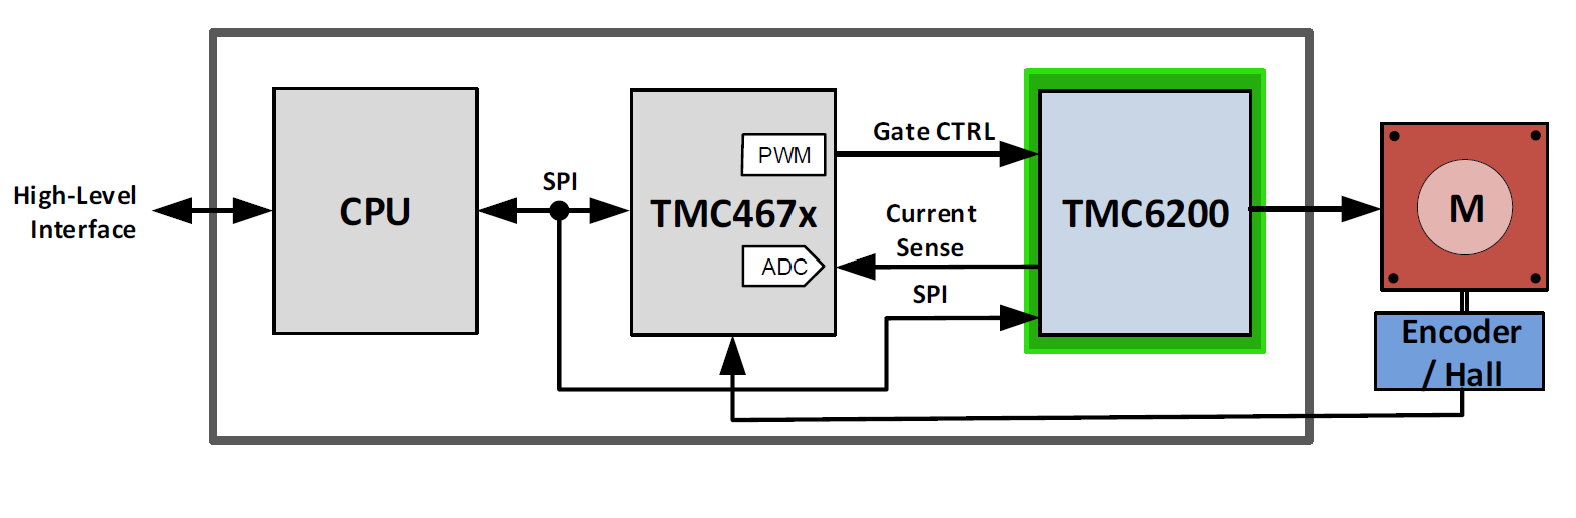
\includegraphics[width=0.8\textwidth]{graphics/Blockdiagramm_TMC4671_und_TMC6200}
	\caption{Blockschaltbild Konfiguration IC's mit BLDC und Encoder}
	\label{fig:Blockdiagramm_TMC4671_und_TMC6200}
\end{figure}

Es wurde darauf geachtet, dass der Aufbau des Prints so gut wie möglich dem Testaufbau entspricht. Im Folgenden wird deshab ein detailierteres Blockschaltbild gezeigt, welches den Aufbau eher nach Funktionen beschreibt, siehe dazu Abbildung \ref{fig:Blockdiagramm_Motorengruppe}. Darin eingezeichnet sind die verwendeten Refernzboards.

\begin{figure}[h!]
	\centering
	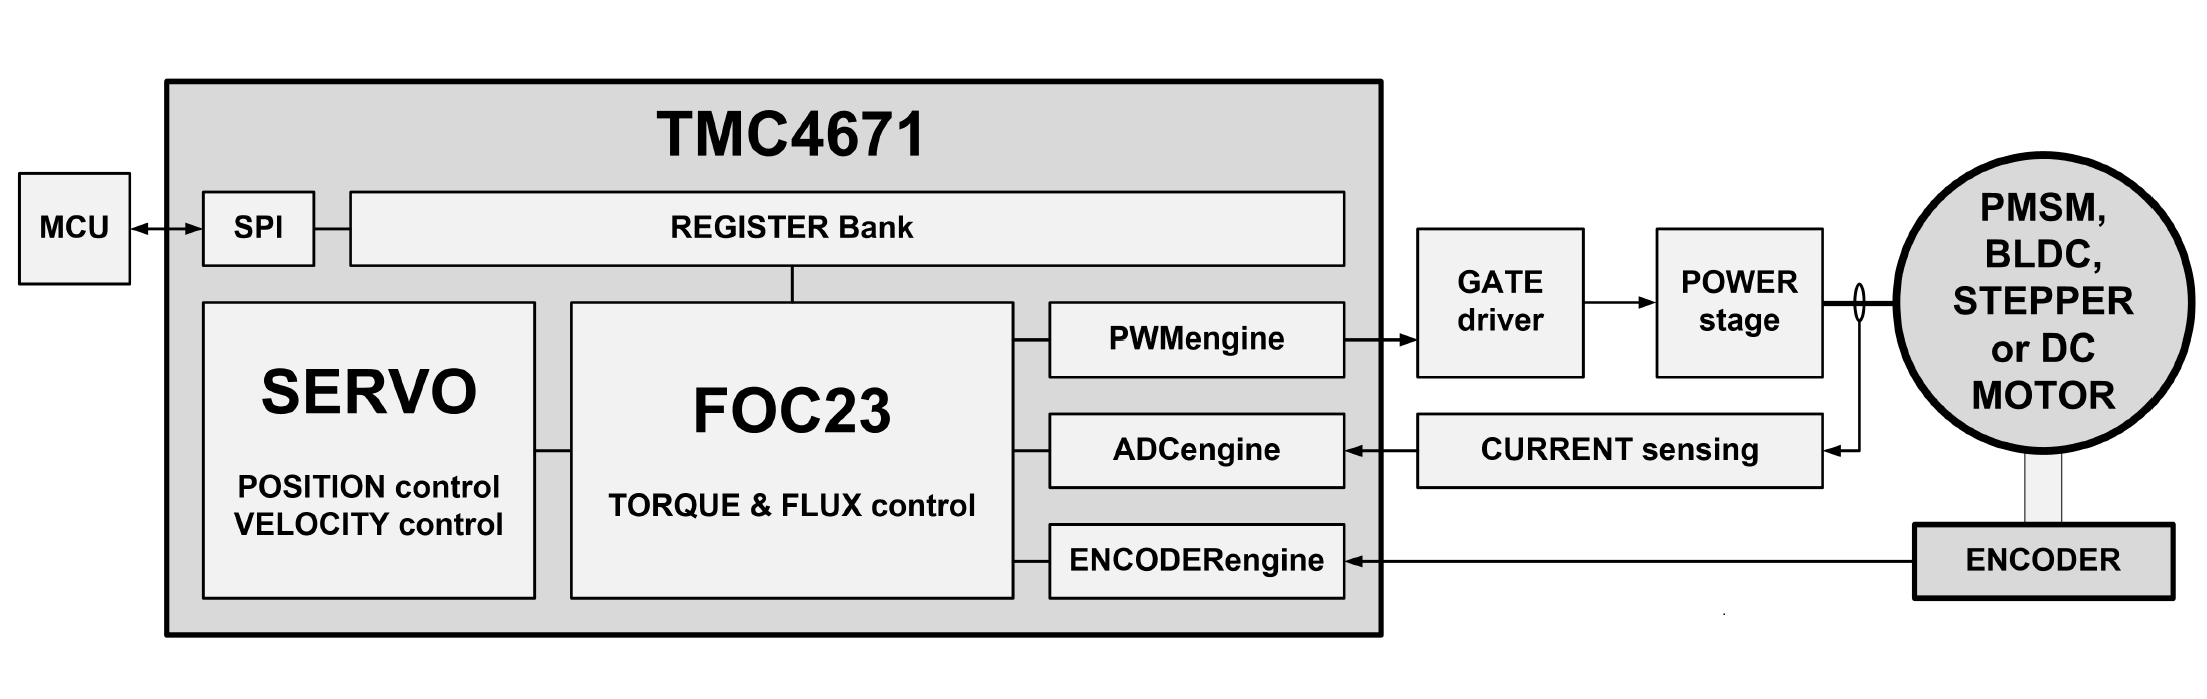
\includegraphics[width=0.8\textwidth]{graphics/Blockdiagramm_Motorengruppe}
	\caption{Blockschaltbild Konfiguration Motorengruppe nach Funktionen.}
	\label{fig:Blockdiagramm_Motorengruppe}
\end{figure}


\begin{tabular}{llll}
TMC4671 & = & Trinamic TMC4671 & FOC-Treiber \\
GATE driver & = & Trinamic TMC6200 & Gate-Treiber \\
POWER stage & = & Trnamic UPS 10A70V & H-Brücke \\
Current sensing & = & UPS 10A70V ==> TMC6200 & Messung Phasenströme \\
PMSM/BLDC & = & Sigmatec AKM22h & BLDC \\
ENCODER & = & CUI devices ATS33 & ABN-Encoder \\
\end{tabular}